    \documentclass[menu.tex]{subfiles}
    \graphicspath{ {images/} }
\begin{document}            
            
            \begin{tabular} {p{3.5cm} p{4cm} p{9cm}}        
        \multicolumn{3} { c }{\begin{LARGE}Menú Semanal 2\end{LARGE}}\\
        \hline
            %---LUNES---%
            \pbox{20cm}{\rule{0pt}{3ex}\begin{large}\textbf{Lunes}\end{large}\\ \rule{0pt}{4ex}Ensalada de pollo con \\ palta \\ 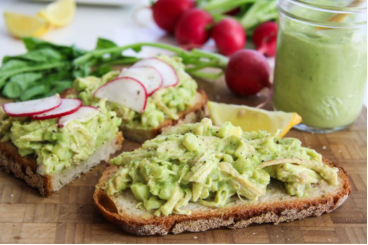
\includegraphics[scale=0.4]{pollo-con-palta} } & 
            \vspace{-2cm}
            \begin{compactitem} 
                \begin{scriptsize}
                    \item Pechuga de pollo troceada
                    \item 1 palta maduro pelado
                    \item 1 manzana pelada
                    \item \nicefrac{1}{4} taza de apio
                    \item \nicefrac{1}{2} taza de cebolla
                    \item Perejil o cilantro
                    \item 2 cucharillas de limón
                    \item Sal
                    \item Pimienta negra molida
                    \item Aceite de oliva
                \end{scriptsize}
            \end{compactitem}&
            \vspace{-2cm}
            Corta la pechuga de pollo en trozos pequeños y sofríe en una sartén con un poco de aceite de oliva. Reserva. Trocea el aguacate, la manzana, el apio y la cebolla. Reserva. Coloca en un bol los trocitos de pollo, aguacate, manzana, apio y cebolla. Con la ayuda de un tenedor machaca el aguacate y mézclalo con el resto de ingredientes hasta formar una especie de pasta. Añade el perejil (o cilantro), el zumo de limón (o lima), la sal y la pimienta y mézclalo bien. Puedes añadir más zumo o incluso aceite de oliva si ves que está demasiado seco. Sirve acompañado de pan, pan tostado o algún tipo de hoja verde para ensalada, como lechuga, berros, verdolaga. Nota: puedes conservarlo en el frigorífico tapado con film transparente.. \\ \hline
            
            \pbox{20cm}{\rule{0pt}{3ex}\begin{large}\textbf{Martes}\end{large}\\ \rule{0pt}{4ex}Ensalada vegetal con carne\\ 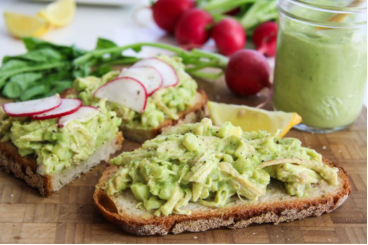
\includegraphics[scale=0.35]{pollo-con-palta} } &
            \vspace{-1.6cm}
            
            \hspace{0.5cm}\begin{footnotesize}Ingredientes (ensalada)\end{footnotesize}
            \begin{compactitem} 
                \begin{scriptsize}
                    \item 1 taza de fresas troceadas
                    \item 1 taza de manzana troceada
                    \item 1 taza de uvas cortadas a la mitad
                    \item 1 taza de naranja troceada
                    \item 2 aguacates troceados
                    \item 1 taza de nueces
                    \item 1 taza de pechuga de pollo troceada
                    \item 1 taza de bacón troceado
                    \item 1 taza de cebolla troceada
                    \item Queso gorgonzola rallado
                    \item Aceite de oliva               
                \end{scriptsize}
            \end{compactitem}
            \hspace{0.5cm}\begin{footnotesize}Ingredientes (aderezo)\end{footnotesize}
            \begin{compactitem} 
                \begin{scriptsize}
                    \item 2 limones maduros
                    \item 4 dientes de ajo machacados
                    \item \nicefrac{1}{2} taza de aceite de oliva
                    \item \nicefrac{1}{4} taza de miel
                    \item 1 cucharilla de mostaza
                    \item Un chorrito de vinagre de vino tinto
                    \item Sal
                \end{scriptsize}
            \end{compactitem} &
            \vspace{-1.6cm}
            Elaboración (ensalada)
    Fríe en una sartén con aceite de oliva la pechuga de pollo y el bacón troceados.
    En un bol grande, mezcla el pollo y el bacón con el resto de ingredientes. Reserva.

    Elaboración (aderezo)
    Exprime los limones en un bol aparte y añade el ajo, el aceite de oliva, la miel, la mostaza, el vinagre y la sal.
    Si el gusto no te convence, añade más sal o miel para adaptarlo a tu paladar.
    Sirve la ensalada en platos individuales y deja que cada comensal se aliñe su ensalada con la cantidad de aderezo que desee.\\ \hline
            
            \pbox{20cm}{\textbf{\textit{Miércoles}} \\ Tacos en base de \\ tortillas y en base \\ vegetal} & Ingredientes & Sobre una tortilla integral coloque carne molida cocinada, vegetales, tomate, cebolla y un poco de palta. Puede preparar los tacos sobre 2 hojas grandes de lechuga, de este modo se reduce significativamente la cantidad de calorías. \\ \hline
            
            \pbox{20cm}{\textbf{\textit{Jueves}} \\ Pastel de carote, \\ brócoli o berenjenas} & Ingredientes & Coloque en una bandeja una fila de carotes o berenjenas cortados en rodajas o brócoli cocido picado. Cubra esta capa con huevo, coloque jamón, vegetales y queso rallado. Cubra nuevamente con carotes, berenjenas o brócoli, De este modo coloque capas hasta formar un pastel del tamaño que le agrade y hornee. \\ \hline
            
            \pbox{20cm}{\textbf{\textit{Viernes}} \\ Berenjenas rebozadas} & Ingredientes & Corte las berenjenas en lonjas y úntelas en una preparación que incluya huevo, sal y una pizca de pimienta, cocínelas en un poco de aceite de oliva o en aerosol. \\ \hline
            
            \pbox{20cm}{\textbf{\textit{Sábado}} \\ Ensalada Cesar} & Ingredientes & Mezcle las verduras de su preferencia con huevos, queso en cuadrados, jamón o enrollado de pollo, aceitunas y carne en trocitos o pollo desmenuzado, coloque salsa cesar light (de cualquier marca) para decorar y sazonar. \\ \hline

            \newpage        
    \end{tabular}
    \end{document}
